\chapter{Implementación de la solución}

Este capítulo...


\section{Implementación: Biblioteca Malva}

Dada la complejidad del problema, se contempló desde el inicio del proyecto la utilización de un \emph{framework} para el desarrollo del algoritmo evolutivo. De esta forma, se logra una implementación robusta y flexible. 

Como se detalló en el marco teórico, existen varias opciones disponibles para seleccionar un \emph{framework} para AEs. Por las particularidades del problema planteado, existen ciertos requerimientos a la hora de seleccionar un \emph{framework}, entre los que se destacan:

\begin{itemize}
	\item Código abierto y gratuito: Al ser un proyecto de investigación de índole académico es conveniente que no existan costos económicos asociados. Además, es importante que se cuente con el código abierto con el fin de introducir modificaciones en el código base o corregir errores.
	\item Algoritmo genético: El \emph{framework} debe facilitar el desarrollo de un algoritmo genético ya que es la base en la que se sustenta el proyecto.
	\item Algoritmo paralelo: Por la complejidad del problema y el alto consumo de recursos computacionales que insume el proceso de evaluación de solciones utilizando simulaciones de SUMO, es fundamental que el \emph{framework} incluya la opción de ejecución en paralelo. Si no cuenta con esta funcionalidad nativa, es deseable al menos que exista la posibilidad de modificar el código base para agregarla.
	\item Plataforma: Es requerido que el \emph{framework} se pueda ejecutar en la plataforma de computación de alto desempeño Cluster FING cuyo sistema operativo es Linux CentOs, ya que es donde se realiza el análisis experimental del trabajo. 
	\item Confiabilidad: Es deseable que el \emph{framework} sea lo suficientemente estable como para tener confianza de que el algoritmo funcionará de manera correcta. Se valorará muy positivamente que existan casos de éxito usando el \emph{framework}, la existencia de documentación accesible, ejemplos de código desarrollado, etc.
	\item Lenguaje: Es deseable que el framework esté desarrollado en C++ o Java ,por la experiencia que el equipo de desarrollo cuenta en estos lenguajes. 
	\item Multiobjetivo: Es deseable (aunque no requerido) que el framework soporte algoritmos multiobjetivo; no es requerido porque la función que se quiere implementar es sencilla y puede usarse una agregación lineal de los objetivos.
\end{itemize} 

Luego de analizar los puntos anteriores, se seleccionó la biblioteca Malva para la implementación del algoritmo evolutivo. A continuación se detalla su funcionamiento y características.

Como se explicó anteriormente, Malva \citep {Malva} surge como una variante del proyecto Mallba \citep{Mallba}. Malva propone la actualización, mejora y desarrollo de Mallba como un proyecto de código abierto colaborativo.  Su objetivo es proveer varios esqueletos de heurísticas de optimización que puedan ser utilizados y extendidos de manera fácil y eficiente. Los esqueletos se basan en separar dos conceptos: el problema concreto que se quiere resolver y el método utilizado para resolverlo. Por lo tanto, un esqueleto se puede ver como una instancia de una plantilla genérica para resolver un problema particular, manteniendo todas las funcionalidades genéricas.

Malva utiliza el lenguaje C++, con el objetivo de brindar modularidad y flexibilidad. Los esqueletos se ofrecen como un conjunto de clases \emph{requeridas} que el usuario deberá modificar para adaptarlo a su problema, y clases \emph{provistas} que incluyen todos los aspectos internos del esqueleto siendo  independientes del problema particular. Entre los algoritmos provistos se encuentran los algoritmos genéticos,algoritmo  CHC \citep{CHC} y otros.


\section{Especificación del Algoritmo Genético utilizado}
Se utiliza el algoritmo genético provisto por la biblioteca  Malva llamado "NewGA", con las modificaciones detalladas en la sección anterior. El siguiente esquema describe el funcionamiento del algoritmo utilizado:

\begin{algorithm}[H]
	\caption{Algoritmo Genético de Malva. }
	\label{alg:algoritmo_genetico_malva}
	\begin{algorithmic} [1] 
		{
			\STATE \texttt{t} = 0
			\STATE {Inicializar( P(t))}
			\STATE {Evaluar estructuras en (P(t))}			
			\WHILE {\text{No terminar}}
			\STATE \texttt{t}++		
			\STATE {Seleccionar C(t) de P(t-1)}	
			\STATE {Recombinar estructuras en C(t) formando C'(t)}				
			\STATE {Mutar estructuras en C'(t) formando C''(t)}		
			\STATE {Evaluar estructuras en C''(t) generando un hilo de ejecucion por cada una}					
			\STATE {Consolidar valores de la evaluacion}								
			\STATE {Reemplazar P(t) de C''(t) y P(t-1)}								
			\ENDWHILE
		}
	\end{algorithmic}
	
\end{algorithm}

A continuación se realiza un resumen de las características del algoritmo implementado, que en la siguiente sección serán descritas en detalle:
\begin{itemize}
	
	\item Se aplica un modelo de algoritmo evolutivo paralelo, utilizando el esquema maestro-esclavo, donde en cada iteración el maestro genera un hilo por cada evaluación de la función de \emph{fitness} y luego espera a la terminación de todos los hilos para consolidar los datos. 
	\item Se considera una formulación multiobjetivo del problema, que intenta optimizar tanto la velocidad promedio de vehículos como la de ómnibus, teniendo cada componente un peso específico en la combinación lineal utilizada para definir la función de \emph{fitness}.
	\item Representación del cromosoma: Es un vector de números naturales que representan la duración de las fases de los semáforos y el \emph{offset} para todos los semáforos del Corredor Garzón.
	\item Cruzamiento y mutación: Se implementa una variante del cruzamiento de un punto específico para este problema y se utilizan dos tipos de mutación para modificar la duración de fase y el \emph{offset} de los semáforos.
	\item Selección y reemplazo: Reemplaza padres por hijos. La selección de los padres se realiza por el método de torneo de tres individuos y la selección de hijos por el método de ruleta.
	
\end{itemize}

\subsection{Representación del cromosoma}

Como se explicó en el marco teórico, el problema de sincronización de semáforos puede ser resuelto optimizando diferentes parámetros. Entre estos parámetros se encuentran la duración de fase, de ciclo y el \emph{offset}. Dependiendo de cuáles se seleccionen deberán ser incluidos en la representación del cromosoma.

Para la solución propuesta se contempla tanto la duración de fase como el \emph{offset}. El cromosoma se agrupa lógicamente en cruces, siendo el valor de cada gen la duración de una
fase en un cruce, además se agrega para cada cruce el valor del \emph{offset}. Se utiliza un vector de números naturales para favorecer la claridad en el desarrollo y la facilidad a la hora de aplicar los operadores. Por este motivo el tamaño del cromosoma depende de la cantidad de cruces y de la cantidad de fases que incluya cada cruce. Con esta representación se busca una optimización global de todo el sistema y no individualmente para cada cruce, lo cual es fundamental para mejorar la velocidad promedio del Corredor Garzón y del resto de las calles que lo cruzan.

En la representación del cromosoma se omiten las luces amarillas ya que no modifican los tiempos reales del paso de vehículos.

\begin{figure}[h]
	\centering
	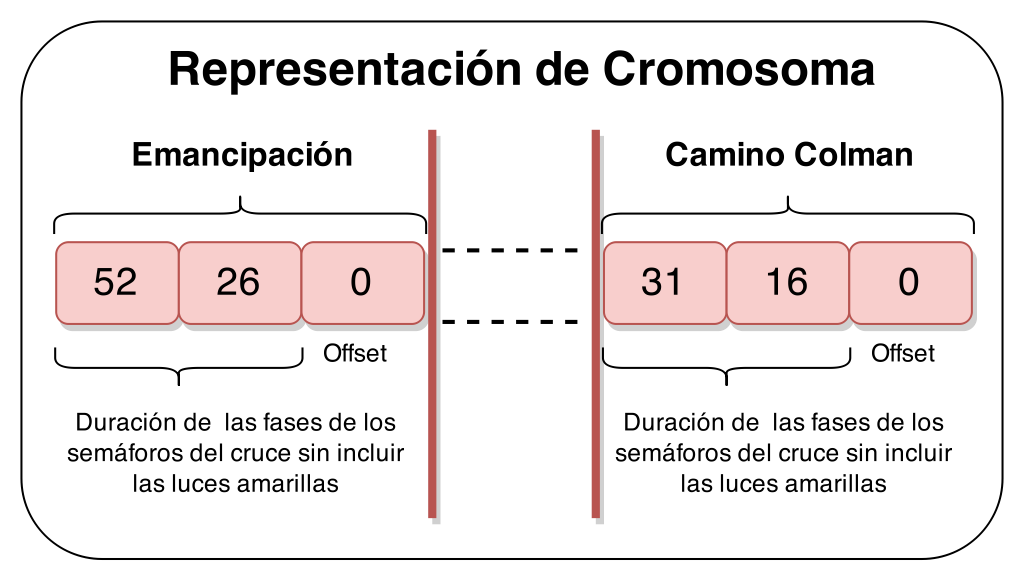
\includegraphics[width=0.7\linewidth]{Figures/cromosoma1}
	\caption{Cromosoma de dos cruces}
	\label{fig:cromosoma1}
\end{figure}

Es importante que el algoritmo evolutivo genere solamente soluciones factibles, por lo tanto se tiene especial cuidado al ejecutar los operadores de cruzamiento y mutación.

\begin{figure}[H]
	\centering
	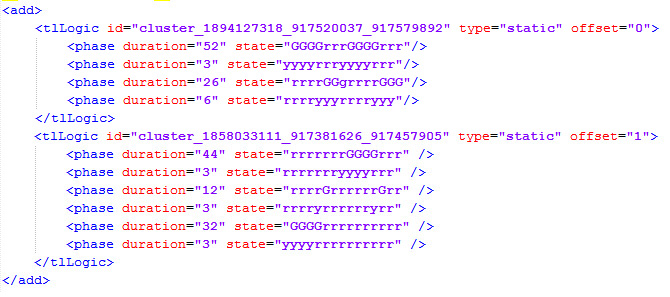
\includegraphics[width=\linewidth]{Figures/rep_sumo2}
	\caption{Representación de Sumo}
	\label{fig:rep_sumo}
\end{figure}

La Figura \ref{fig:rep_sumo} muestra el archivo de configuración de semáforos que utiliza el simulador SUMO para el cromosoma anterior, donde se representan las fases. Por ejemplo la fase \emph{GGGGrrrGGGGrrr} indica la secuencia de luces y su duración de 52 segundos, \emph{G} indica la luz verde, \emph{r} la roja, \emph{y} el Amarillo. El valor del \emph{offset} indica el inicio de la fase. 

La Figura \ref{fig:sem_numerados} presenta la numeración de los semáforos que se corresponden con la primera fase de este ejemplo, donde cada posición de la secuencia \emph{estado} se corresponde con un color en particular. 

\newpage
Por tanto para el estado \emph{GGGGrrrGGGGrrr} se tiene que:
\begin{itemize}
	\item GGGG se corresponde a 1, 2, 3 y 4. 
	\item rrr a 5, 6 y 7. 
	\item GGGG a 8, 9, 10 y 11. 
	\item rrr a 12, 13 y 14. 
\end{itemize}

\begin{figure}[H]
	\centering
	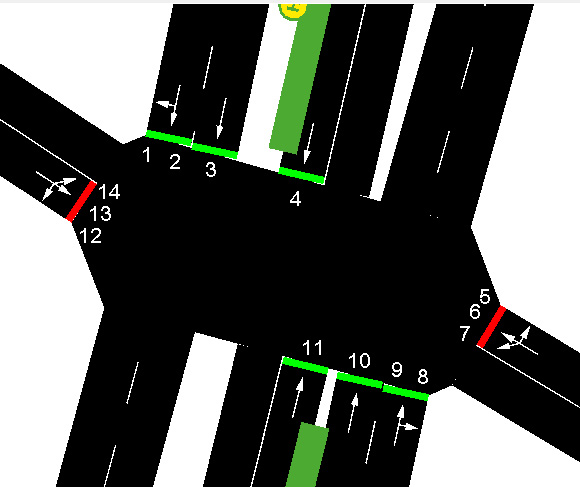
\includegraphics[width=0.7\linewidth]{Figures/semaforos_numerado}
	\caption[Representación de una fase de los semáforos para un cruce.]{Representación de una fase de los semáforos para un cruce. Cada número se corresponde a una letra en la secuencia de \emph{state} del archivo de configuración del simulador SUMO.}
	\label{fig:sem_numerados}
\end{figure}

\subsection{Población inicial}

Para la inicialización de la población se toma como referencia
la configuración obtenida a partir de los datos de la realidad,  luego para cada cruce se varían las duraciones de las fases de manera aleatoria entre un rango de valores configurable. Además se selecciona la fase inicial aleatoriamente entre la cantidad de fases del cruce.

\subsection{Función \emph{fitness}}


La evaluación de un individuo se realiza generando un archivo con la configuración de los semáforos en base a su cromosoma y ejecutando el simulador SUMO utilizando esta configuración para obtener los datos necesarios para calcular el \emph{fitness}.

Se emplea una función multiobjetivo usando combinación lineal de la velocidad de los ómnibus y del resto de los vehículos, ya que es un método sencillo y adecuado cuando son menos de tres objetivos. El \emph{fitness} se calcula como una suma ponderada, con los pesos fijados a priori.

\begin{equation}
\label{eq:funcion_fitness_generica}
F(x) = \sum_{i=1}^{n}{w_i}{f_i}(x)
\end{equation}

Se selecciona como objetivo la velocidad promedio de los ómnibus (vpb) y la velocidad promedio del resto de los vehículos (vpv). Esta métrica fue elegida pues es más adecuada para realizar las comparaciones con la realidad. Por ejemplo la cantidad de vehículos que completan su viaje, la duración promedio del recorrido o el tiempo de simulación son todas métricas que podrían usarse pero no son útiles a la hora de realizar comparaciones con la realidad.

La siguiente es la fórmula de \emph{fitness} utilizada, donde \emph{x} e \emph{y} indican los pesos que se especifican en la función. En una primera instancia se establece x = y = 1, más adelante se experimentará con otros pesos.

\begin{equation}
\label{eq:funcion_fitness}
f = x.vpb + y.vpv
\end{equation}



Se plantea optimizar la velocidad promedio de los vehículos en toda la red vial, de manera global, esto quiere decir que se busca una mejor velocidad promedio tanto en autos que van por Garzón como aquellos que circulan por los cruces o calles paralelas. La optimización global es fundamental, ya que si cada cruce se optimiza individualmente podría generar problemas de congestión en otras zonas.

\subsection{Operadores}
\subsubsection{Operador de Cruzamiento}
Se utiliza cruzamiento de un punto, seleccionando del cromosoma una posición aleatoria entre dos cruces como punto de corte, por tanto si un tramo del corredor tiene un buen comportamiento se intenta mantener esa propiedad. En el escenario que plantea la siguiente Figura, los padres cuentan con tres cruces. Se elige un punto de corte aleatoriamente entre dos cruces y se generan los hijos que son una combinación de los padres.

\begin{figure}[H]
	\centering
	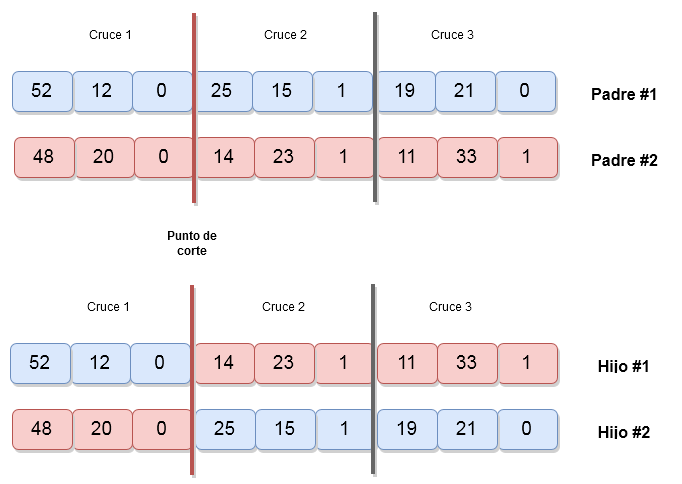
\includegraphics[width=8cm]{Figures/alg_cruzamiento}
	\caption{Visualización del cruzamiento entre individuos.}
	\label{fig:op_cruzamiento}
\end{figure}



\subsubsection{Operador de Mutación}
Se implementaron dos tipos de mutación:
\begin{itemize}
	
	\item Mutación de duración de fase: para cada fase de cada cruce se modifica su duración sumando o restando una cantidad dada de segundos, con una probabilidad dada. Teniendo en cuenta que el valor obtenido se encuentre dentro de un rango especificado para que no se produzcan casos irreales como un cruce de menos de 5 segundos.
	
	\item Mutación del \emph{offset}: Se elige aleatoriamente una fase con la cual va a comenzar el cruce con una probabilidad dada.
\end{itemize}

\subsubsection{Selección y reemplazo}
Se  utilizan los operadores y criterios provistos por el algoritmo genético newGA de Malva. La selección de padres se realiza por el método de torneo de tres individuos y la selección de hijos por el método de ruleta. La política de reemplazo indica que tanto padres como hijos pueden ser parte de la siguiente generación (no solamente los hijos), por lo que existe reemplazo de padres por hijos.

\subsubsection{Parámetros del algoritmo}
Los parámetros específicos del algoritmo se establecen en el siguiente capítulo, donde se realiza un análisis experimental para encontrar los más adecuados. Estos parámetros son: número de generaciones, tamaño de población, probabilidad de cruzamiento y de mutación.


\section{Modelo de paralelismo e implementación}

Uno de los requisitos planteados al inicio del presente trabajo era la creación de un algoritmo genético que soportara paralelismo, con el objetivo de reducir los tiempos de ejecución. El motivo principal fue que los escenarios planteados se consideraron complejos y que utilizarían gran cantidad de recursos computacionales. Para este propósito, se utilizó como código base el algoritmo genético provisto por la biblioteca Malva llamado NewGA. Este código fue modificado para que el algoritmo soportara la ejecución en paralelo, específicamente se desarrolló una nueva forma de evaluar a los individuos, generando un hilo de ejecución por cada individuo.

Se utilizó el método maestro-esclavo para el modelo de paralelismo. El proceso maestro se encarga de la mayoría de las etapas del algoritmo evolutivo, al comenzar, inicializa la población y se encarga de distribuir la evaluación de los individuos hacia los esclavos, creando un hilo de ejecución por cada esclavo. Luego el proceso maestro espera a que las evaluaciones terminen para obtener los valores de \emph{fitness} de los esclavos. Una vez obtenidos los valores, selecciona a los mejores individuos y le aplica los operadores de cruzamiento y mutación. Para finalizar ejecuta el criterio de reemplazo para generar la siguiente población. Mientras, los esclavos se encargan solamente de obtener el individuo enviado por el maestro y de efectuar la evaluación del individuo, que corresponde a ejecutar el simulador y obtener los datos de salida.

En el capítulo siguiente, en la sección de análisis experimental se realiza un estudio de la eficiencia computacional del algoritmo genético paralelo, para comparar los tiempos de ejecución entre la versión paralela y en serie.